\documentclass[1p]{elsarticle}

\usepackage{amsmath}
\usepackage{amsfonts}

\usepackage{subcaption}

\usepackage{epstopdf}

\title{Data-driven Reduction of Multiscale Stochastic Dynamical Systems }

\author[PrincetonCBE]{C.J.~Dsilva}
\ead{cdsilva@princeton.edu}

\author[YaleMath]{R.~Talmon}
\ead{ronen.talmon@yale.edu}

\author[PrincetonCBE]{C.W.~Gear}
\ead{wgear@princeton.edu}

\author[YaleMath]{R.R.~Coifman}
\ead{coifman@math.yale.edu}

\author[PrincetonCBE, PrincetonPACM]{I.G.~Kevrekidis\corref{cor1}}
\ead{yannis@princeton.edu}

\address[PrincetonCBE]{Department of Chemical and Biological Engineering, Princton University, Princeton, New Jersey, 08544, USA}
\address[YaleMath]{Department of Mathematics, Yale University, New Haven, Connecticut, 06520, USA}
\address[PrincetonPACM]{Program in Applied and Computational Mathematics, Princton University, Princeton, New Jersey, 08544, USA}

\cortext[cor1]{Corresponding author}


\begin{document}

\begin{abstract}

\begin{itemize}

\item Link between data mining and dynamical systems analysis

\item Extracting/reducing an SDE system to its slow variables using the Mahalanobis graph and NIVs

\item Full mathematical analysis of the slow variable reduction procedure, including necessary conditions for accurate recovery of the intrinsic variables and a framework for empirically setting the algorithm parameters

\end{itemize}

\end{abstract}


\begin{keyword}
 
\end{keyword}

\maketitle

\section{Introduction}

\section{Theory}

\subsection{Multiscale SDEs}

Given a system of SDEs with separation of timescales, we want to recover slow variable(s) even when the fast variables are have large variations.

Consider the following system of SDEs:
\begin{equation} \label{eq:fast_slow_SDE}
\begin{aligned}
dx &= adt + dW^1\\
dy &= -\frac{y}{\epsilon} dt + \frac{1}{\sqrt{\epsilon}} dW^2
\end{aligned}
\end{equation}

So $x$ is the slow variable, and $y$ is a fast noise whose equilibrium measure is bounded and $\mathcal{O}(1)$.
%
We assume that the saturation time of fast scale  of the SDE is smaller than the other relevant timescales.
%
We would like to recover $x$ using data-driven techniques.

We would like to note that the ratio of the drift and diffusion terms in the $y$ equation is essential.
%
We need the square of the diffusivity to be of the same order as the drift.
%
If the diffusivity is too large, the equilibrium measure of $y$ will be unbounded.
%
Conversely, if the diffusivity is too small, the equilibrium measure of $y$ will go to 0.

%TODO: should we write the SDE in a more general form?

\subsection{Nonlinear Intrinsic Variables}

The goal of NIVs is to recover ``intrinsic'' variables that are independent of the measurement/observation function.
%
We define intrinsic variables as those variables which have uncoupled noise with unit variance,
i.e., the intrinsic variables $X^1, \dots, X^n$ are governed by the following SDEs:
\begin{equation} \label{eq:NIV_formulation}
dX^i = a(X) dt + dW^i
\end{equation}
where $X = \begin{bmatrix} X^1 & X^2 & \cdots & X^n \end{bmatrix}^T$.

These same conditions for uncoupled noises with unit variance will allow us to recover the slow variable(s) from data with multiple timescales. 
%
We want to emphasize the link between multiscale SDEs and NIVs: NIVs rescales the noises, so that the ``fast'' variables become small.
%
Consider the SDE in \eqref{eq:fast_slow_SDE}, and let $y = \frac{z}{\sqrt{\epsilon}}$. 
%
Then
\begin{equation}
\begin{aligned}
dx &= adt + dW_1\\
dz &= -\frac{z}{\epsilon} dt +  dW_2
\end{aligned}
\end{equation}
%
Therefore, $z$ is a stochastic variable whose diffusion is unity, and so $x$ and $z$ are the ``intrinsic variables'' for the underlying SDE.
%
However, the equilibrium measure of $z$ is $\mathcal{O}(\epsilon)$, and so when $\epsilon \ll 1$, $z \ll x$, and so we will recover $x$ (the slow variable). 
%
In general, we want to recover the slow variable(s) even when the observations of the underlying intrinsic stochastic process are obstructed by a {\em nonlinear} measurement function. 

\subsection{Errors and Estimation}

\begin{itemize}
\item Error and estimation analysis of NIVs (remark that applies to more general settings): give conditions/bounds when we can recover the intrinsic slow variable
%
\item Empirical configuration/demonstration of the method, how to use the analysis to set the parameters in the algorithm
\end{itemize}

Given $X$ governed by the SDE in \eqref{eq:NIV_formulation}, we can sample ``bursts'' around a point $X_0$ in order to estimate the local covariance of the noise. 

These clouds will be distributed 

\begin{equation}
X \sim \mathcal{N}\left( X_0, \delta t I \right)
\end{equation}


We now consider a function $\mathbf{f}: \mathbb{R}^n \mapsto \mathbb{R}^m$.
%
Let $f^i(X)$ denote the $i^{th}$ entry of $\mathbf{f}$, and let $f^i_j(X) = \frac{\partial f^i}{\partial X^j}$.
%
By Taylor expansion around $X=X_0$,
%
\begin{eqnarray}
\hat{C}(X_0) &=& \delta t J_1 J_1^T 
+ \frac{\delta t^2}{2} \left[ J_1 J_3^T + J_3 J_1^T  
+ \frac{3}{2} J_2 J_2^T 
-\frac{1 }{2} J_2 1 1^T J_2^T \right]
+ \mathcal{O} (\delta t^3) %\\
%&=& \delta t J_1 J_1^T 
%+ \frac{\delta t^2}{2} U \Sigma V
%+ \mathcal{O} (\delta t^3)
\end{eqnarray}
where
\begin{equation}
\begin{aligned}
J_1(X_0) &= \begin{bmatrix}
f_1^1 & f_2^1 & \dots & f_n^1 \\
\vdots & \vdots & \cdots & \vdots \\
f_1^m & f_2^m & \dots & f_n^m
\end{bmatrix}\\
%
J_2(X_0) &= \begin{bmatrix}
f_{11}^1 & f_{22}^1 & \dots & f_{nn}^1 \\
\vdots & \vdots & \cdots & \vdots \\
f_{11}^m & f_{22}^m & \dots & f_{nn}^m
\end{bmatrix}\\
%
J_3(X_0) &= \begin{bmatrix}
f_{111}^1 & f_{222}^1 & \dots & f_{nnn}^1 \\
\vdots & \vdots & \cdots & \vdots \\
f_{111}^m & f_{222}^m & \dots & f_{nnn}^m
\end{bmatrix}
\end{aligned}
\end{equation}
%
In this equation, we see what we expect (a linear function of the variance, due to the gradient of $f$) and a second (higher-order) term arising from the curvature and third derivative of $f$.
%
The importance of this second term increases as the curvature increases, as well as when $\delta t$ increases. 



Then
\begin{equation}
\hat{C}^{-1}(X_0) \approx \frac{1}{\delta t} \left( J J^T \right)^{-1} - A
\end{equation}
%
where 
\begin{equation}
A = \frac{1}{2} (J_1 J_1^T)^{-1} U \left(\Sigma^{-1} + \frac{\delta t}{2} V \left( J_1 J_1^T \right)^{-1} U \right)^{-1} V \left( J_1 J_1^T \right)^{-1}
\end{equation}
and
\begin{equation}
U \Sigma V = J_1 J_3^T + J_3 J_1^T + \frac{3}{2} J_2 J_2^T -\frac{1 }{2} J_2 1 1^T J_2^T 
\end{equation}
$A$ is a function of the first-, second-, and third-order derivatives of $\mathbf{f}$.


We now approximate the distances $\| X_2 - X_1 \|$.
%
Let $g = f^{-1}: \mathbb{R}^m \mapsto \mathbb{R}^n$, and let $Y_1 = f(X_1)$, and $Y_2 = f(X_2)$.
%
Again, we let $g_j^i = \frac{\partial g^i}{\partial Y^j}$.
%
Then, by Taylor expansion, we obtain
\begin{equation} \label{eq:taylor_expansion}
\begin{aligned}
&\| X_2 - X_1 \|^2 \\
\le&  \left| \frac{1}{2} (Y_2 - Y_1 )^T ((J J^T)^{-1} (Y_1) + (J J^T)^{-1}(Y_2)) (Y_2 - Y_1 ) \right| \\
& + n \left( \left| K_1 K_2 \right| + \left| \frac{ K_2^2}{4} \right|  + \left| \frac{K_1 K_3}{3} \right|  \right) \| Y_2 - Y_1 \| ^4  \\
& + \mathcal{O} (\|Y_1 - Y_2 \|^6 ) 
\end{aligned}
\end{equation}
%
where
%
\begin{equation}
\begin{aligned}
K_1 &= \sup_{i,j,Y} |g_j^i(Y)|\\
K_2 &= \sup_{i,j,k,Y} |g_{jk}^i(Y)|\\
K_3 &= \sup_{i,j,k,l,Y} |g_{jkl}^i(Y)|
\end{aligned}
\end{equation}

Substituting our estimate of the covariance into \eqref{eq:taylor_expansion}, we obtain
\begin{equation}
\begin{aligned}
&\| X_2 - X_1 \|^2 \\
\approx &  \frac{1}{2} (Y_2 - Y_1)^T \left((J J^T)^{-1}(Y_1)  + (J J^T)^{-1}(Y_2) \right) (Y_2 - Y_1) \\
& - \frac{\delta t}{2} (Y_2 - Y_1)^T \left( A(Y_1) + A(Y_2) \right) (Y_2 - Y_1)\\
& + n \left( \left| K_1 K_2 \right| + \left| \frac{ K_2^2}{4} \right|  + \left| \frac{K_1 K_3}{3} \right|  \right) \| Y_2 - Y_1 \| ^4  \\
& + \mathcal{O} (\|Y_1 - Y_2 \|^6 ) 
\end{aligned}
\end{equation}
%
We want the first term in this expression to dominate.

From \eqref{eq:taylor_expansion}, we can see that the squared {\em intrinsic} distance $\| X_2 - X_1 \|^2$, is a function of $\|Y_2 - Y_1\|$ and $\delta t$. 
%
If the first term in the expansion dominates, then $\|X_2 - X_1 \|^2$ should be independent of $\delta t$, and should vary quadratically with $\| Y_2 - Y_1\|$. 
%
We can find such a regime empirically (by plotting $\| X_2 - X_1 \|^2$ as a function of $\delta t$ and $\|Y_2 - Y_1\|$), and select a kernel distance where both conditions hold.


\begin{figure}
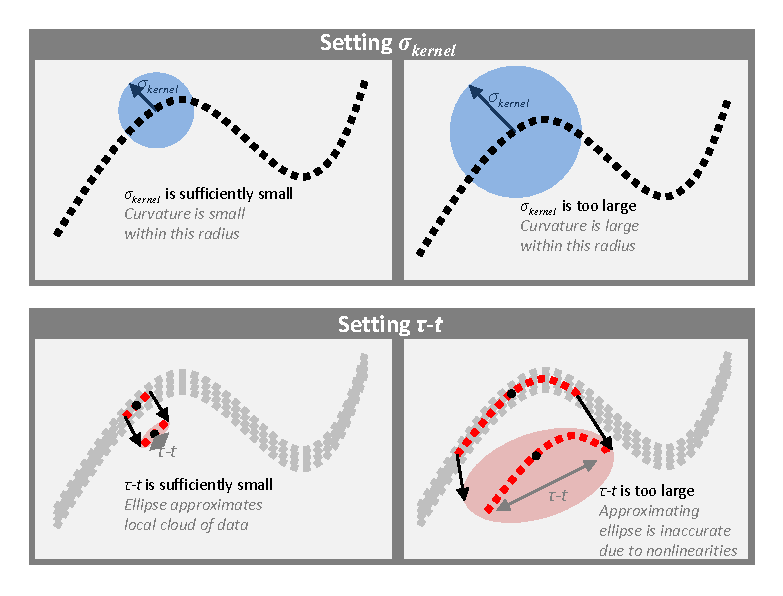
\includegraphics[width=\textwidth]{schematic}
\caption{Illustration of how to choose $\delta t$ and $\sigma_{kernel}$ appropriately. The data shows the evolution of the ``fast'' variable at a fixed value of the ``slow'' variable.  We must choose both parameters so that the curvature effects and other nonlinearities are negligable. }
\label{fig:schematic}
\end{figure}

\section{Results}
 
Define the following two-dimensional system of SDEs
\begin{eqnarray} \label{eq:init_data}
dX(1) &=& 3 dt + dW_1 \\ 
dX(2) &=& \frac{-X(2)}{\epsilon} dt + dW_2 
\end{eqnarray}
where $W_1, W_2$ are independent Brownian motions, and $\epsilon \ll 1$.
%

Let
\begin{eqnarray}\label{eq:transformed_data}
f^1(X) &=& X(1) + \frac{ X(2)^2}{\epsilon} \\
f^2(X) &=& \frac{X(2)}{\sqrt{\epsilon}}
\end{eqnarray}
Therefore, the two ``intrinsic variables'' $X(1), X(2)$ have been nonlinearly transformed and rescaled such that the new variables $f^1(X), f^2(X)$ are both $\mathcal{O}(1)$, even though $X(1)$ is the ``fast'' variable. 
%
The inverse function $g = f^{-1}$ is
\begin{eqnarray}
g^1(Y) &=& Y(1) - Y(2)^2 \\
g^2(Y) &=& Y(2) \sqrt{\epsilon}
\end{eqnarray}
%
Data from a simulation is shown in Figure~\ref{fig:initial_data}.

\begin{figure}[h]
\begin{subfigure}{0.5\textwidth}
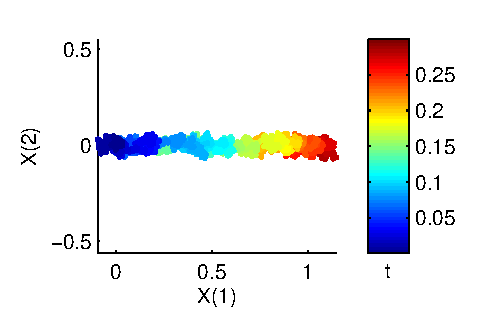
\includegraphics[width=\textwidth]{data_init}
\caption{}
\end{subfigure}
\begin{subfigure}{0.5\textwidth}
\includegraphics[width=\textwidth]{data_transformed}
\caption{}
\end{subfigure}
\caption{(a) The original data, simulated from \eqref{eq:init_data} with $\epsilon = 10^{-3}$. We take $3000$ timesteps with $dt = 10^{-4}$ (b) The data from (a), transformed according to \eqref{eq:transformed_data}. }
\label{fig:initial_data}
\end{figure}

\subsection{NIVs versus DMAPS}

We first want to demonstrate the utility of NIVs over DMAPS. 
%
We compute the first (nontrivial) NIV and DMAPS coordinate using the data in Figure~\ref{fig:initial_data}(b). 
%
The results are shown in Figure~\ref{fig:NIV_versus_DMAPS}.
%
NIV accurately recovers the slow variable (the coloring in Figure~\ref{fig:NIV_versus_DMAPS}(a) is consistent with the coloring in Figure~\ref{fig:initial_data}(b)). 
%
In contrast, DMAPS does not recover the slow variable. 

\begin{figure}[h]
\begin{subfigure}{0.5\textwidth}
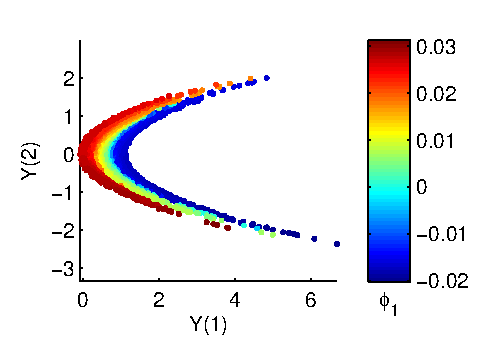
\includegraphics[width=\textwidth]{data_transformed_colored_NIV}
\caption{}
\end{subfigure}
\begin{subfigure}{0.5\textwidth}
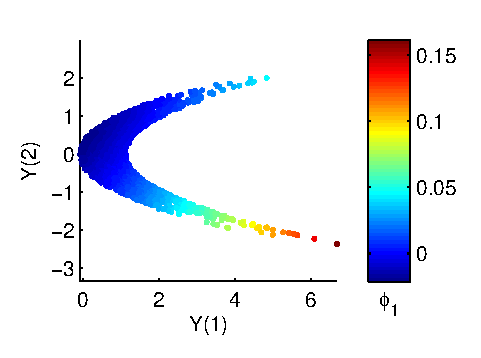
\includegraphics[width=\textwidth]{data_transformed_colored_DMAPS}
\caption{}
\end{subfigure}
\caption{(a) The data from Figure~\ref{fig:initial_data}(b), colored by the first NIV (we take $\sigma_{kernel} = 0.01$, and $\delta t = 10^{-9}$). Note that we recover the slow variable. (b) The data from Figure~\ref{fig:initial_data}(b), colored by the first DMAPS variable (we take $\sigma_{kernel} = 0.01$). Note that we do {\em not} recover the slow variable.}
\label{fig:NIV_versus_DMAPS}
\end{figure}

\subsection{Determining Appropriate Parameters}

We would like to demonstrate how we can {\em empirically} determine the appropriate parameters $\delta t$ and $\sigma_{kernel}$ so that we can accurately recover the slow variable(s).

For the system in \eqref{eq:init_data} and \eqref{eq:transformed_data}, the three relevant quantities for NIVs are 
\begin{itemize}
\item The linearized approximation to the distance,
%
\begin{equation}
(Y_2 - Y_1)^T (JJ^T)^{-1} (Y_2 - Y_1) 
\approx \mathcal{O} \left(  \frac{1}{2} \left( 2 + \epsilon + \sqrt{ 9 + 2 \epsilon + \epsilon^2}\right) \Delta Y^2\right) 
\end{equation}
where $\Delta Y =  \|Y_2 - Y_1\|$

\item The error from the {\em estimation} of the covariance.
%
This is
\begin{equation}
\frac{\delta t}{2} (Y_2 - Y_1)^T A (Y_2 - Y_1) \approx \mathcal{O} \left( \frac{38 \delta t}{\epsilon ^2 + 2 \delta t}\Delta Y^2 \right)
\end{equation}

\item The errors from the {\em truncation} of the Taylor expansion for the Mahalanobis distance, which is 
\begin{equation}
n \left( \left| K_1 K_2 \right| + \left| \frac{ K_2^2}{4} \right|  + \left| \frac{K_1 K_3}{3} \right|  \right) \| Y_2 - Y_1 \| ^4 \approx \mathcal{O} \left( 10 \Delta Y^4  \right) 
\end{equation}

\end{itemize}
%
We can plot each of these quantities analytically as a function of $\delta t$ and $\|Y_2 - Y_1\|$. 
%
The results are shown in Figure~\ref{fig:empirical_estimation}(a)~and~(c). 
%
In practice, for more complex SDEs, we cannot write down the three terms analytically.
%
We can only measure the sum of the three terms; this is the estimate of the intrinsic distance that we calculate, $\|X_2 - X_1 \|^2_{est}$.
%
This is also shown in Figure~\ref{fig:empirical_estimation}(a)~and~(c).
%
Clearly, when higher-order terms become important corresponds to a ``kink'' in the plots. 
%
We can also plot the empirical estimates of $\| X_2 - X_1 \|^2_{est}$ obtained from simulation data, as a function of $\delta t$ and $\| Y_2 - Y_1 \|$.
%
This is shown in Figure~\ref{fig:empirical_estimation}(b)~and~(d). 
%
The same ``kink'' is evident in these plots at approximately the same position as the analytical plots. 
%
Therefore, we choose $\delta t$ and a $\sigma_{kernel}$ which corresponds to a $\|X_2 - X_1 \|_{est}^2$ value {\em before} the kink. 
%
For this particular example, we take $\delta t = 10^{-9}$ and $\sigma_{kernel} = 0.01$, which allows us to accurately recover the slow variable. 

\begin{figure}[h]
\begin{subfigure}{0.5\textwidth}
\includegraphics[width=\textwidth]{errors_function_dt}
\caption{}
\end{subfigure}
\begin{subfigure}{0.5\textwidth}
\includegraphics[width=\textwidth]{empirical_totaldist_function_dt}
\caption{}
\end{subfigure}
\begin{subfigure}{0.5\textwidth}
\includegraphics[width=\textwidth]{errors_function_dy}
\caption{}
\end{subfigure}
\begin{subfigure}{0.5\textwidth}
\includegraphics[width=\textwidth]{empirical_totaldist_function_dy}
\caption{}
\end{subfigure}
\caption{(a) Total estimated distance (black) and the three separate terms in the estimated distance, as a function of $\delta t$. The linearized approximation is in blue, the error from the covariance estimation is in green, and the error from the truncation of the distance expansion is in red. 
%
(b) Empirical estimation of total distance as a function of $\delta t$, with $\|Y_2 - Y_1 \|^2 = 0.01$.  
%
(c) Total estimated distance (black) and the three separate terms in the estimated distance, as a function of $\|Y_2 - Y_1\|$. The linearized approximation is in blue, the error from the covariance estimation is in green, and the error from the truncation of the distance expansion is in red. 
%
(d) Empirical estimation of total distance as a function of $\|Y_2 - Y_1\|$, with $\delta t =  10^{-9}$. The red line corresponds to the quadratic $\|X_2 - X_1 \|^2_{est} \propto \|Y_2 - Y_1 \|^2$.}
\label{fig:empirical_estimation}
\end{figure}

\begin{figure}
\begin{subfigure}{0.5\textwidth}
\includegraphics[width=\textwidth]{changing_parameters_error_terms_1}
\caption{}
\end{subfigure}
\begin{subfigure}{0.5\textwidth}
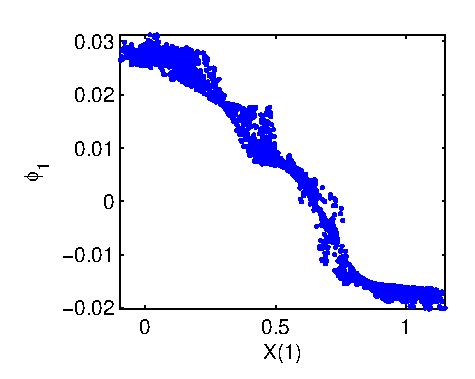
\includegraphics[width=\textwidth]{changing_parameters_NIV_corr_1}
\caption{}
\end{subfigure}

\begin{subfigure}{0.5\textwidth}
\includegraphics[width=\textwidth]{changing_parameters_error_terms_2}
\caption{}
\end{subfigure}
\begin{subfigure}{0.5\textwidth}
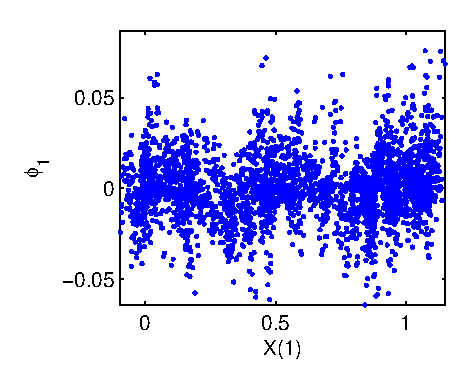
\includegraphics[width=\textwidth]{changing_parameters_NIV_corr_2}
\caption{}
\end{subfigure}

\begin{subfigure}{0.5\textwidth}
\includegraphics[width=\textwidth]{changing_parameters_error_terms_3}
\caption{}
\end{subfigure}
\begin{subfigure}{0.5\textwidth}
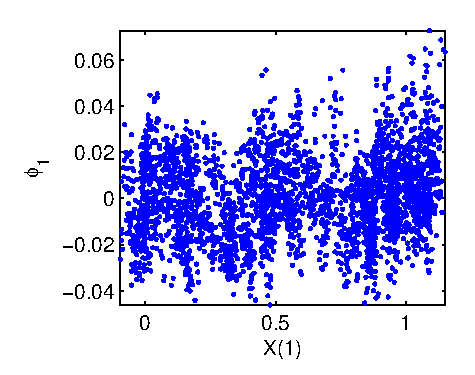
\includegraphics[width=\textwidth]{changing_parameters_NIV_corr_3}
\caption{}
\end{subfigure}

\caption{ Error analysis and recovery of the slow variable for three different simulation configurations. (a, b) $\sigma_{kernel} = 10^{-2}$, $\delta t = 10^{-9}$, (c, d) $\sigma_{kernel} = 10^{2}$, $\delta t = 10^{-9}$ (e, f) $\sigma_{kernel} = 10^{-2}$, $\delta t = 10^{-5}$.  (a, c, e) The three separate terms in the estimated distance, as a function of $\|Y_2 - Y_1\|$. The linearized approximation is in blue, the error from the covariance estimation is in green, and the error from the truncation of the distance expansion is in red. The blue circle indicates the value of $\sigma_{kernel}$ used in the diffusion maps calculations. (b, d, f) The first NIV, obtained from the transformed data $Y$, versus the slow variable $X(1)$. Note that we only recover the slow variable $X(1)$ when the linearized approximation dominates the other two error terms in the distance function at the scale of $\sigma_{kernel}$. }

\end{figure}

\subsection{Recovery of Fast Variable}

The size of the ``burst'' we take also affects the recovery of the fast variable, even when there is no nonlinear transformation.
%
When the time scale of the burst is smaller than that of the equilibration time of the fast variable, the estimated covariance is constant and the fast variable is collapsed significantly relative to the slow variable.
%
This means that the fast variable is recovered {\em very} far down in the DMAPS eigenvectors.
%
However, if the time scale of the burst is {\em longer} than the saturation time of the fast variable, the estimated covariance changes: the variance in the slow direction continues to grow, while the variance in the fast direction is fixed.
%
This means that the collapse of the fast variable is less pronounced relative to the slow variable, and the fast variable is recovered in a higher eigenvector. 

We again consider the SDE system from \eqref{eq:init_data}, and consider the transformation
\begin{eqnarray}\label{eq:transformed_data2}
h^1(X) &=& X(1)  \\
h^2(X) &=& \frac{X(2)}{\sqrt{\epsilon}}
\end{eqnarray}
%
Unlike previously, there is no nonlinear component to the transformation, only a rescaling that makes the noise in the ``fast'' direction larger. 

Figure~\ref{fig:vary_burst} shows data collected from simulation of \eqref{eq:transformed_data2}.
%
Different timescales were used to simulate the bursts and estimate the local covariance. 
%
We can see that, when the timescale is less than the saturation time of the fast variable (the first two plots), the fast variable is recovered deep in the eigenvalue spectrum (eigenvector 14).
%
However when the timescale exceeds the saturation time of the fast variable (the third plot), the fast variable moves up in the eigenvalue spectrum (eigenvector 8).

\begin{figure}[h]
%\begin{subfigure}{0.5\textwidth}
%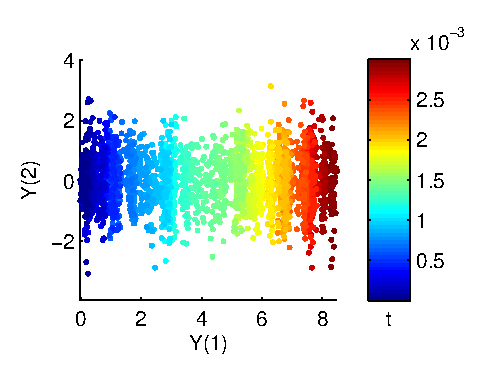
\includegraphics[width=\textwidth]{dat_varyburst}
%\caption{}
%\end{subfigure}
%
\begin{subfigure}{0.3\textwidth}
\includegraphics[width=\textwidth]{data_withburst_1}
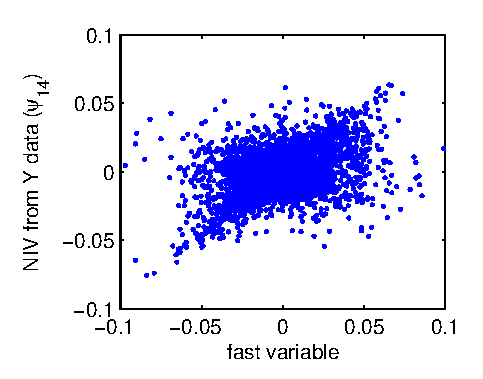
\includegraphics[width=\textwidth]{fast_var_corr_1}
\caption{}
\end{subfigure}
\begin{subfigure}{0.3\textwidth}
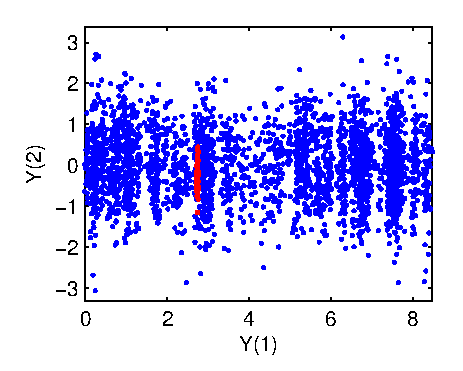
\includegraphics[width=\textwidth]{data_withburst_2}
\includegraphics[width=\textwidth]{fast_var_corr_2}
\caption{}
\end{subfigure}
\begin{subfigure}{0.3\textwidth}
\includegraphics[width=\textwidth]{data_withburst_3}
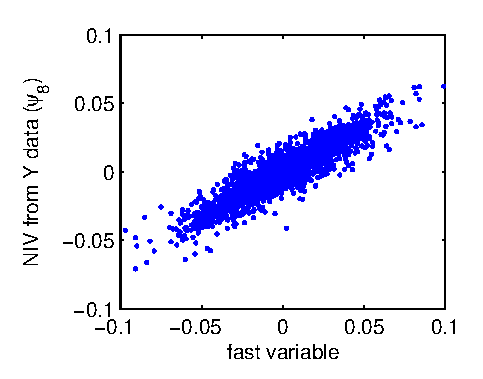
\includegraphics[width=\textwidth]{fast_var_corr_3}
\caption{}
\end{subfigure}
\caption{
(a) Top: data in blue, simulated from \eqref{eq:init_data} and \eqref{eq:transformed_data2}, with representative burst in red.  
%
Bottom: correlation between NIV coordinate and fast variable. 
%
(b) Top: data in blue, with representative burst in red.  
%
Bottom: correlation between NIV coordinate and fast variable. 
%
(c) Top: data in blue, with representative burst in red.  
%
Bottom: correlation between NIV coordinate and fast variable. }
\label{fig:vary_burst}
\end{figure}

\section{Conclusion}

We showed that in certain cases (when we do {\em not} have a simulator where we can change $\delta t$), the data cannot be processed as-is (we cannot find the right kernel scale given a fixed $\delta t$ such that we can accurately recover the slow variable). 

If the cloud of samples is too big then we can observe the cloud of clouds (and those clouds can be histograms, Fourier, scattering, etc.) as a way to get smaller clouds. 


Richardson extrapolation could allow us to get an estimate of a second-order term in the covariance estimation, thereby locally approximating the function using a quadratic form, rather than a linear form,  which can lead to a better/improved/more accurate ``Mahalanobis'' metric. 



\end{document}
